\chapter{Dynamics}

\section{Two pulleys}
\begin{wrapfigure}{o}{0.5\textwidth}
  % \centering
  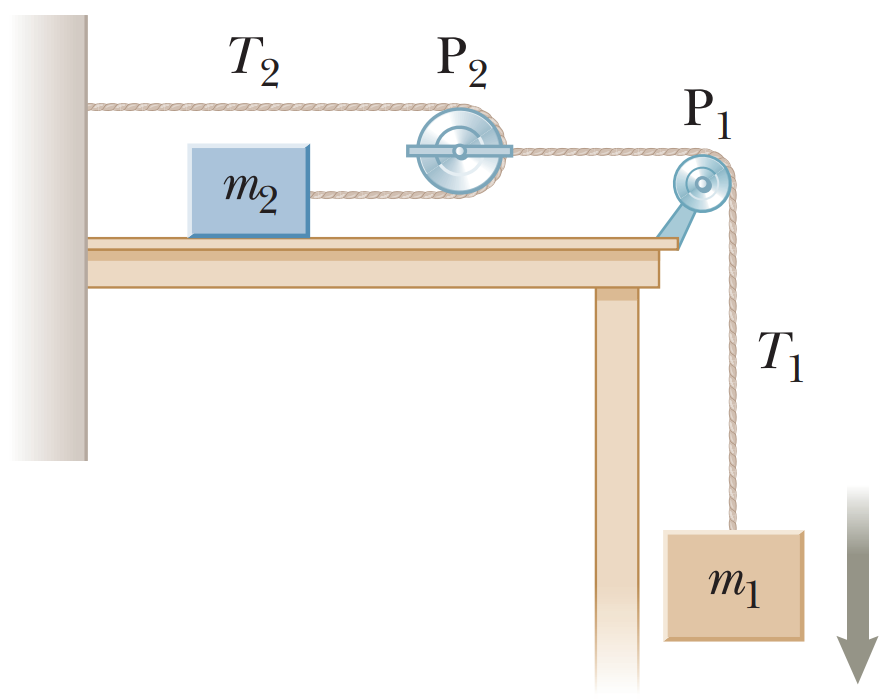
\includegraphics{assets/twopulleys.png}
  \caption{A two-pulley system}
  \label{fig:twopulleys}
\end{wrapfigure}

\begin{problem}
  In \cref{fig:twopulleys}, a mass \(m_1\) hangs from a massless string
  that passes over a very light fixed pulley \(P_1\).
  The same string is connected to a second light pulley \(P_2\). A
  second string passes around \(P_2\) with one end
  attached to a wall and the other to another mass \(m_2\) on a
  frictionless, horizontal table.
  If \(a_1\) and \(a_2\) are the accelerations of \(m_1\) and
  \(m_2\) respectively, deduce the tensions \(T_1\) and \(T_2\) in \(m_1\) and
  \(m_2\) (respectively) in terms of \(m_1\), \(m_2\) and \(g\).
\end{problem}

Taking downwards as \(+y\), and by \term{Newton's Third Law},
\begin{align}
  \label{eq:m1a1}
  m_1a_1 &= m_1g-T_1 \\
  m_2a_2 &= T_2
  \label{eq:m2a2}
\end{align}
We observe also that \(P_2\) is being pulled on by \(P_1\) and
\(m_2\). Since its
mass is negligible, the net force acting on it must be zero.
\begin{equation}
  0 = 2T_2 - T_1
  \label{eq:t1t2}
\end{equation}
We also observe that \(P_2\) coils twice for every coil \(P_1\) makes, so
\begin{equation}
  2a_1 = a_2
  \label{eq:a1a2}
\end{equation}

Substituting \cref{eq:t1t2} and \cref{eq:a1a2} into \cref{eq:m1a1},
\begin{align*}
  m_1g - 2T_2 &= m_1a_1 \\
  &= \f{m_1a_2}{2} \\
  &= \f{m_1T_2}{2m_2} \\
  \therefore\; T_2\ab(\f{m_1}{2m_2}+2) &= m_1g \\
  T_2 &= \f{2m_1m_2g}{m_1 + 4m_2}
\end{align*}

Recalling \cref{eq:t1t2},
\begin{align*}
  T_1 &= 2T_2 \\
  &= \f{4m_1m_2g}{m_1+4m_2}
\end{align*}

\section{See-saw}
\begin{problem}
  Two people are standing on a \qty{2.0}{\metre} long platform, one at
  each end. The platform floats parallel
  to the ground on a cushion of air, like a hovercraft. One person
  throws a \qty{6.0}{\kg} ball
  to the other, who catches it. The ball travels nearly horizontally.
  Excluding the ball, the total mass of the platform and people is
  \qty{120}{\kg}. Because of the throw, this \qty{120}{\kg} mass
  recoils. How far
  does it move before coming to rest again?
\end{problem}

Assuming the platform to be uniform and both people to be of the same
mass, we define
\begin{itemize}
  \item \(m_b\) and \(m_p\) to be the masses of the ball and the
    people and platform combined, respectively.
  \item \(\mv{v}_b\) and \(\mv{v}_p\) to be the velocities of the ball
    and the platform (with people), respectively.
  \item \(x\) to be the recoil length of the people and platform.
\end{itemize}
Using the \term{principle of conservation of momentum},
\begin{equation}
  m_b\mv{v}_b + m_p\mv{v}_p = 0
  \label{eq:pcomball}
\end{equation}
Since the time taken for the ball to pass over from the thrower to the catcher
is equal to that for the platform to recoil,
\begin{equation}
  \f{2.0}{\mv{v}_p - \mv{v}_b} = \f{x}{\mv{v}_p}
  \label{eq:timetaken}
\end{equation}
Substituting \cref{eq:pcomball} into \cref{eq:timetaken},
\begin{align*}
  \f{2.0}{21\mv{v}_p} &= \f{x}{\mv{v}_p}\\
  x &= \lf{2.0}{21} \\
  &= \hil{\qty{0.095}{\metre}}
\end{align*}

\section{Two carts}
\begin{problem}
  The supposed figure here shows the momentum--time graph for a
  collision between
  two carts with masses of \qty{1.0}{\kg} and \qty{3.0}{\kg} respectively.
  Show that the collision of the carts obey the principle of conservation
  of linear momentum.
\end{problem}

The \term{principle of conservation of linear momentum} states that
\(\Delta\mv{p}_1 = -\Delta\mv{p}_2\).
\begin{align*}
  \Delta\mv{p}_1 &= 0.0 - 2.0 \\
  &= \qty{-2.0}{\kg\m\per\second} \\
  \Delta\mv{p}_2 &= 1.0 - \ab(-1.0) \\
  &= \qty{2.0}{\kg\m\per\second} \\
  \sum\Delta\mv{p} &= -2.0 + 2.0 \\
  &= \hil{\qty{0}{\kg\m\per\second}}
\end{align*}

\begin{problem}
  Show that the force acting on cart 1 by cart 2 is equal to that
  acting on cart 2 by cart 1 during collision.
\end{problem}
According to the graph, the time taken for the collision is the same
for cart 1 on cart 2 and vice versa. Since
\begin{align*}
  \Delta\mv{p}_1 &= -\Delta\mv{p}_2 \\
  \Rightarrow \mv{J}_1 &= -\mv{J}_2 \\
  \odv{\mv{J}_1}{t} &= -\odv{\mv{J}_2}{t} \\
  \therefore\; \mv{F}_1 &= -\mv{F}_2
\end{align*}

\begin{problem}
  Explain if this collision is an elastic, inelastic or perfectly
  inelastic collision.
\end{problem}
The \term{elasticity} of a collision is dependent on the loss of kinetic energy
from the system after the collision.
\begin{align*}
  \text{KE} &= \f{1}{2}m\mv{v}^2 \\
  &= \f{\mv{p}^2}{2m} \\
  \sum \text{KE} &= \f{\ab(2.0)^2}{2\times 1.0} +
  \f{\ab(-1.0)^2}{2\times 3.0} \\
  &= \qty{2.2}{\joule} \\
  \sum \text{KE}' &= \f{\ab(0.0)^2}{2\times 1.0} +
  \f{\ab(1.0)^2}{2\times 3.0} \\
  &= \qty{0.2}{\joule}
\end{align*}
Since \(\Delta\text{KE} < 0\), some (but not all) kinetic energy was
lost from the system. The collision is \hil{inelastic}.

\section{Putty lump}
\begin{wrapfigure}{o}{0.4\textwidth}
  % \centering
  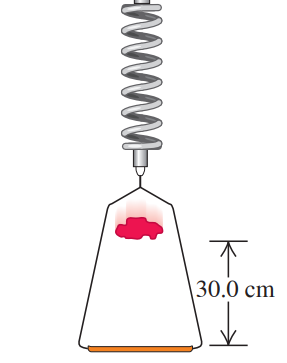
\includegraphics[scale=0.5]{assets/puttylump.png}
  \caption{Suspended frame containing putty lump}
  \label{fig:puttylump}
\end{wrapfigure}

\begin{problem}
  In \cref{fig:puttylump}, a \qty{0.150}{\kg} frame, when suspended from a coil
  spring, stretches the spring \qty{0.0700}{\metre}. A \qty{0.200}{\kg} lump of
  putty is dropped from rest onto the frame from a height of \qty{30.0}{\cm}.
  Find the maximum distance the frame moves downward from its
  initial equilibrium position.
\end{problem}

We define our terms:
\begin{itemize}
  \item \(m_f\) and \(m_p\) are the masses of the frame and putty
    lump respectively.
  \item \(\mv{u}_p\) is the velocity of the putty lump just before
    hitting the frame.
  \item \(\mv{v}\) is the velocity of the putty lump and frame
    combined, after the collision.
  \item \(k\) is the spring constant of the coil spring.
  \item \(x_0\) is the original stretched length of the spring.
\end{itemize}

We can first find the spring constant, since the weight of the frame
provides the elastic force in the spring.
\begin{align*}
  m_f\,\mv{g} &= kx_0 \\
  k &= \f{m_f\,\mv{g}}{x_0} \\
  &= \f{0.150\times 9.81}{0.070} \\
  &= \qty{21.02}{\newton\per\metre}
\end{align*}

Taking downwards as \(+y\), the terminal velocity of the putty is
\begin{align*}
  \mv{u}_p &= \sqrt{2g\mv{s}_p} \\
  &= \sqrt{2\ab(-9.81)\ab(-0.300)} \\
  &= \qty{2.426}{\metre\per\second}
\end{align*}
The collision between the lump of putty and frame is perfectly
inelastic because the putty is assumed to
have adhered to the frame. By the \term{principle of conservation of momentum},
\begin{align*}
  m_p\mv{u}_p + 0 &= \mv{v}\ab(m_p + m_f) \\
  \mv{v} &= \f{m_p\mv{u}_p}{m_p + m_f}
\end{align*}

The gravitational potential energy lost due to the descent and the
kinetic energy
gained will contribute to the stretching of the spring. Taking \(\mv{s}\) to be
the maximum length of the spring,
\begin{align*}
  m\mv{g}\ab(\mv{s}-x_0) + \f{1}{2}\ab(m_p + m_f)\mv{v}^2 &=
  \f{1}{2}k\mv{s}^2 \\
  \f{k}{2}\mv{s}^2 - m\mv{g}\mv{s} + m\mv{g}x_0 -
  \f{\mv{v}^2\ab(m_p+m_f)}{2} &= 0 \\
  \mv{s} &= \f{m\mv{g} + \sqrt{\ab(m\mv{g})^2 - 2k\ab[mx_0\mv{g} -
  \f{1}{2}\ab(m_p + m_f)\mv{v}^2]}}{k} \\
  \mv{s} &= \qty{0.340}{\metre} \\
  \therefore\;\mv{s} - x_0 &= \hil{\qty{0.270}{\metre}}
\end{align*}

\section{Rocket fuel}
\begin{problem}
  A rocket of empty mass \(M_0\) carries fuel with an effective mass \(m\).
  The fuel is combusted and ejected out of the rocket at a rate of
  \(\odv{m}{t} = \lambda\)
  with speed \(v_e\) relative to the rocket. Derive the equation of
  motion of a rocket travelling at speed \(v\) inside
  Earth.
\end{problem}

In this problem, the mass of the rocket changes with respect to time.
Let \(M\ab(t)\) be the mass
of the system at any time \(t\), and \(m\ab(t)\) be the mass of the fuel at any
time \(t\).
We can say that
\begin{equation}
  M\ab(t) = M_0 + m\ab(t)
  % \label{eq:systemmass}
\end{equation}

Furthermore, since \(\odv{m}{t}=\lambda\), we can say that
\(\f{m_1 - m_0}{t_1-t_0}\) is true too. Substituting \(t_0 = 0\),
\(t_1 = t\) (at any time \(t\) throughout the fuel's motion), and \(m_1 = 0\),
\begin{equation}
  M\ab(t) = M_0 - \lambda t
  \label{eq:systemmass}
\end{equation}

The momentum of the system (the rocket \it{and} the fuel inside it) is thus
\begin{equation}
  \mv{p}\ab(t) = M\ab(t)\mv{v}_r\ab(t)
  \label{eq:sysp}
\end{equation}
where \(\mv{v}_r\ab(t)\) is the rocket's velocity with respect to time.

Over a short period of time from \(t\) to \(t + \odif{t}\),
a small mass \(\odif{m}\) of fuel is ejected from the rocket with
velocity \(\mv{v}_e\). According to the \term{principle of
conservation of linear momentum},
the momentum of the system at time \(t\) is the momentum of the
rocket and remaining fuel,
added to the momentum of the fuel ejected.
\begin{equation}
  \mv{p}\ab(t + \odif{t}) = M\ab(t+\odif{t})\mv{v}_r\ab(t+\odif{t}) +
  \odif{m}\ab[\mv{v}_e + \mv{v}_r\ab(t+\odif{t})]
  \label{eq:sysp2}
\end{equation}
Since the mass of the system is constant, the mass lost from the
rocket \(\odif{M}\)
is equal to the mass gained in the ejected fuel \(\odif{m}\). With
\(\odif{m} = -\odif{M}\). Rewriting \cref{eq:systemmass}, we get
\begin{equation}
  M = M\ab(t+\odif{t}) + \odif{m} = M\ab(t) + \odif{M} + \odif{m}
  \label{eq:sysm2}
\end{equation}
Substituting \cref{eq:sysm2} into \cref{eq:sysp2}, we get
\begin{align*}
  \mv{p}\ab(t + \odif{t}) &= M\ab(t+\odif{t})\mv{v}_r\ab(t+\odif{t}) +
  \odif{m}\ab[\mv{v}_e + \mv{v}_r\ab(t+\odif{t})] \\
  &= M\ab(t) + \cancel{\odif{M}\mv{v}_r\ab(t+\odif{t})} - \odif{M}\ab[\mv{v}_e +
  \cancel{\mv{v}_r\ab(t+\odif{t})}] \\
  &= M\ab(t)\mv{v}_r\ab(t+\odif{t}) - \odif{M}\mv{v}_e
\end{align*}
Since the external force \(\mv{F}\) acting on the rocket is the
change in momentum
with respect to time,
\begin{align*}
  \mv{F} &= \odv{\mv{p}}{t} \\
  &= \lim_{\odif{t}\to 0} \f{\mv{p}_1 - \mv{p}_0}{\odif{t}} \\
  &= \lim_{\odif{t}\to 0} \f{\ab[M\ab(t)\mv{v}_r\ab(t+\odif{t}) -
    \odif{M}\mv{v}_e] -
  \ab[M\ab(t)\mv{v}_r\ab(t)]}{\odif{t}} \\
  &= M\ab(t)\lim_{\odif{t}\to
  0}\f{\mv{v}\ab(t+\odif{t})-\mv{v}_r\ab(t)}{\odif{t}}-\lim_{\odif{t}\to
  0}\mv{v}_e\odv{M}{t}
\end{align*}

The \hil{external force} acting on the system is therefore
\begin{equation}
  \mv{F} = M\ab(t)\odv{\mv{v}_r}{t} - \mv{v}_e\odv{M}{t}
  \label{eq:fext}
\end{equation}

Taking the movement of the rocket to be in the positive direction,
\(\mv{v}_r = v_r\ii\).
Since the fuel moves in the negative direction,
we can say \(\mv{v}_e = -v_e\ii\), where \(v_e\) is a constant.
\begin{align*}
  \mv{F} = M\ab(t)\odv{v_r}{t} + v_e\odv{M}{t}
\end{align*}

Assuming that there are \it{no external forces} acting on the system,
\begin{align*}
  M\ab(t)\odv{v_r}{t} &= -v_e\odv{M}{t} \\
  \odif{v_r} &= -v_e\f{\odif{M}}{M\ab(t)}
\end{align*}

Solving this differential equation yields
\begin{align*}
  \int_{{v_r}_0}^{{v_r}_1}\odif{v_r} &=
  -v_e\int_{M_0}^{M_1}\f{\odif{M}}{M} \\
  {v_r}_1 - {v_r}_0 &= -v_e\ln\ab(\lf{M_1}{M_0}) \\
  &= v_e\ln\ab(\lf{M_0}{M_1})
\end{align*}
Substituting in \({v_r}_0 = v\) and \(M_1 = M_0 - \lambda t\) to the
above yields
\begin{equation}
  v_r = v + v_e\ln\f{M_0}{M_0 - \lambda t}
  \label{eq:rocketans}
\end{equation}

\section{Falling sand}
\begin{problem}
  Sand falls through a hole in a sandbag at a rate of
  \qty{0.100}{\kg\per\second} and lands
  on the pan of a weighing machine directly below. The hole is
  \qty{1.00}{\metre} above the pan.
  Find the velocity of the sand just before it hits the pan.
\end{problem}

Neglecting air resistance, the sand is in \term{free fall}. The
\term{terminal velocity} is thus
\(v = \sqrt{2gh}\), where \(g\) is the gravitational constant and
\(h\) is the height from which
the sand has fallen.
\begin{align*}
  v &= \sqrt{2 g h} \\
  &= \sqrt{2 \times \ab(-9.81) \times \ab(-1.00)} \\
  &= \hil{\qty{4.43}{\metre\per\second}}
\end{align*}

\begin{problem}
  Assuming the sand stops when it hits the pan, what is the change
  of momentum of the sand per second due to the impact?
\end{problem}
We know that \(\Delta\mv{p} = m\Delta\mv{v}\).
\begin{align*}
  \Delta\mv{p} \text{ (per second)} &= m\Delta\mv{v} \\
  &= 0.100 \times 4.43 \\
  &= \hil{\qty{0.443}{\kg\metre\per\second}}
\end{align*}

\begin{problem}
  What is the force on the pan due to the impact alone?
\end{problem}
We know that \(\mv{F} = \odv{\mv{p}}{t}\). therefore, \(\mv{F} =
\lf{\Delta\mv{p}}{\Delta t} = \hil{\qty{0.443}{\newton}}\).

\begin{problem}
  If the total mass of the sand is \qty{1.00}{\kg}, what is the
  reading of the balance (in \unit{\kg}) when the last grain of sand
  hits the pan?
\end{problem}
The reading on a weighing balance is \(\mv{F}/g\), where \(\mv{F}\)
is the net force exerted on the surface.
\begin{align*}
  \mv{F} &= -\ab[-\mv{g} + \ab(-\mv{F}_\text{sand--pan})] \\
  &= 9.81 + 0.443 \\
  &= \qty{10.253}{\newton}\\
  \text{reading} &= \lf{10.253}{g} \\
  &= \hil{\qty{1.05}{\kg}}
\end{align*}

\section{Colliding atoms}
\begin{problem}
  A neon atom (\(m = \qty{20.0}{\dalton}\)) makes a perfectly elastic
  collision with another atom at rest.
  After the impact, the neon atom travels away at a \qty{55.6}{\degree}
  angle from its original direction
  and the unknown atom travels away at a \qty{-50.0}{\degree} angle.
  What is the mass of the unknown atom, in \unit{\dalton}?
\end{problem}

Let
\begin{itemize}
  \item \(\mv{u}\) be the initial horizontal velocity of the neon
    atom, assuming that there is always an initial horizontal
    velocity that produces such a glancing collision.
  \item \(m_1\) and \(m_2\) be the masses of the neon atom and
    unknown atom respectively.
  \item \(\alpha\) and \(\beta\) be the angles of deflection of the
    neon atom and unknown atom respectively.
  \item \(\mv{v}_1\) and \(\mv{v}_2\) be the final velocities of the
    neon atom and unknown atom respectively.
\end{itemize}
The goal here is to obtain an expression for \(m_2\), in terms of the
given factors
\(m_1\), \(\alpha\), and \(\beta\).

The \term{law of conservation of momentum} dictates that, for a
head-on collision,
\begin{equation}
  m_1\mv{u}_1 + m_2\mv{u}_2 = m_1\mv{v}_1 + m_2\mv{v}_2
\end{equation}

Applying this in the horizontal and vertical directions respectively,
\begin{align}
  \label{eq:pconvx}
  m_1\mv{u} &= m_1\mv{v}_1 \cos\alpha + m_2\mv{v}_2 \cos \beta \\
  0 &= m_1\mv{v}_1 \sin \alpha - m_2\mv{v}_2 \sin \beta
  \label{eq:pconvy}
\end{align}

Since the collision was \term{elastic}, the relative speed of approach
is equal to the relative speed of separation.
\begin{equation}
  \mv{u} = \mv{v}_2 \cos \beta - \mv{v}_1 \cos \alpha
  \label{eq:approachspeed}
\end{equation}

We can rewrite \cref{eq:pconvy} as
\begin{equation}
  m_2\mv{v}_2 = \dfrac{m_1\mv{v}_1\sin\alpha}{\sin\beta}
  \label{eq:mv2}
\end{equation}

Substituting the result from \cref{eq:mv2} into \cref{eq:pconvx}, we obtain
\begin{align*}
  m_1\mv{u} &= m_1\mv{v}_1\cos\alpha +
  \dfrac{m_1\mv{v_1}\sin\alpha}{\sin\beta}\cos\beta \\
\end{align*}
\begin{equation}
  \mv{u} = \mv{v}_1\ab(\cos\alpha + \sin\alpha\cot\beta)
  \label{eq:uv1}
\end{equation}

Similarly, from \cref{eq:approachspeed}, we can also write
\begin{equation}
  \mv{v}_2 = \dfrac{\mv{u} + \mv{v}_1\cos\alpha}{\cos\beta}
  \label{eq:v2}
\end{equation}

Substituting \cref{eq:v2} into \cref{eq:mv2}, we obtain
\begin{align*}
  m_2 &= \dfrac{m_1\mv{v}_1\sin\alpha}{\sin\beta} \cdot \dfrac{1}{\mv{v}_2} \\
  &=
  \dfrac{m_1\mv{v}_1\sin\alpha}{\sin\beta}\cdot\dfrac{\cos\beta}{\mv{u}
  + \mv{v}_1\cos\alpha} \\
\end{align*}
\begin{equation}
  \therefore\; m_2
  =\dfrac{m_1\mv{v}_1\sin\alpha\cot\beta}{\mv{u}+\mv{v}_1\cos\alpha}
  \label{eq:m2}
\end{equation}

Returning from \cref{eq:uv1} and substituting into \cref{eq:m2}, we
finally get
\begin{equation}
  m_2 = \dfrac{m_1\sin\alpha\cot\beta}{2\cos\alpha + \sin\alpha\cot\beta}
\end{equation}

Using this result (after long last!), we obtain:
\begin{align*}
  m_2 &= \dfrac{m_1\sin\alpha\cot\beta}{2\cos\alpha + \sin\alpha\cot\beta} \\
  &=
  \ab|\frac{20\sin\qty{55.6}{\degree}\cot\ab(\qty{-50.0}{\degree})}{2\cos\qty{55.6}{\degree}
  + \sin\qty{55.6}{\degree}\cot\ab(\qty{-50.0}{\degree})}| \\
  &= \hil{\qty{31.6}{\dalton}}
\end{align*}

\section{Rocket explosion}
\begin{problem}
  A rocket is fired vertically upward. At the instant it reaches an
  altitude of \qty{1000}{\metre} and a
  speed of \qty{300}{\metre\per\second}, it explodes into three
  fragments of equal mass. One fragment moves
  upward with a speed of \qty{450}{\metre\per\second} following the
  explosion, while another has a speed of
  \qty{240}{\metre\per\second} eastwards. What is the velocity of the
  last fragment immediately after the explosion?
\end{problem}

Throughout this problem, \(+y\) is northward, and \(+x\) eastward.
The final velocity of the rocket, \(\mv{v}_1\), is
\begin{align*}
  \mv{v}_1 &= \sqrt{\mv{v}_0^2 + 2\mv{a}\mv{s}}\\
  &= \sqrt{\ab(300)^2 + 2\ab(-9.81)(1000)} \\
  &= \qty{265.3}{\metre\per\second}
\end{align*}
Let the three fragments be \(A\), \(B\) and \(C\), each with mass
\(m\). By the \term{law of conservation of momentum}\sidenote{\(\ii\)
and \(\jj\) are unit vectors in the \(x\)-- and \(y\)--directions.},
\begin{align*}
  m(\mv{v}_A + \mv{v}_B + \mv{v}_C) &= -3m\mv{v}_1 \\
  \mv{v}_C &= -3\mv{v}_1 - \ab(\mv{v}_A + \mv{v}_B) \\
  &= -3\ab(v_1\jj) - 450\jj - 240\ii \\
  &= -240\ii - (3v_1 + 450)\jj \\
  \ab|\mv{v}_C| &= \sqrt{\ab(-240)^2 + \ab[-(3v_1+450)]^2}\\
  &= \hil{\qty{831.3}{\metre\per\second}} \\
  \text{direction of } \mv{v}_C &= \arctan\f{3v_1 +450}{240} \\
  &= \hil{\qty{73}{\degree}\text{ south of west}}
\end{align*}

\section{Hydrogen molecules}
\begin{problem}
  When two hydrogen atoms of mass \(m\) combine to form a diatomic
  hydrogen molecule,
  the potential energy of the system after they combine is \(-A\),
  where \(A\) is a positive quantity called the
  \term{binding energy} of the molecule.
  Show that, in a collision that involves only two hydrogen atoms, it
  is impossible to form a hydrogen molecule because momentum and energy
  cannot simultaneously be conserved.
\end{problem}

Let \(\mv{u}_n\) be the initial velocity of the \(n\)--th hydrogen
molecule, and
\(\mv{v}_n\) be its final velocity. Let \(\mv{v}\) be the final
velocity of the
hydrogen molecule formed.

Initially, the total momentum is \(\mv{p} = m\ab(\mv{u}_1 + \mv{u}_2)
= 0\). Since momentum
must be conserved, \(\mv{p}' = 2m\mv{v} = 0\). It follows that
\(\mv{v} = 0\), so
the hydrogen molecule must be at rest after the collision.
\begin{equation}
  \mv{v} = 0
  \label{eq:finalv}
\end{equation}

Initially, the total energy in the system is \(E = \f{1}{2}m{u_1}^2 +
\f{1}{2}m{u_2}^2 = \f{m\ab({u_1}^2 + {u_2}^2)}{2}\).
After the collision, some energy has been converted to potential
energy (due to the aforementioned binding energy),
hence
\begin{equation}
  E' = \f{2mv^2}{2} - A
  \label{eq:finalE}
\end{equation}

Substituting \cref{eq:finalv} into \cref{eq:finalE}, we get \(E' = -A\).
However, since \(E' > A > 0\), \hil{the above finding is contradictory}.

\begin{problem}
  A hydrogen molecule can be formed in a collision involving three
  hydrogen atoms.
  Before such a collision, each of the three atoms has a speed of
  \(\mv{u}=\qty{1.00e4}{\metre\per\second}\). They approach at angles
  of \qty{120}{\degree}
  so that at any instant, the atoms lie at the corners of an
  equilateral triangle.
  The binding energy of hydrogen is \(A = \qty{7.23e-19}{\joule}\), and the mass
  of a hydrogen atom is \(m = \qty{1.67e-27}{\kg}\). Find
  \begin{itemize}
    \item the speed of the resulting hydrogen molecule;
    \item the speed of the remaining hydrogen atom.
  \end{itemize}
\end{problem}

Let the final speed of the hydrogen molecule and hydrogen atom be
\(\mv{v}\) and \(\mv{w}\) respectively,
and let their directions of travel be \(\alpha\) and \(\beta\).
We can apply the \term{law of conservation of momentum} in both the
\(x\) and \(y\) directions,
taking rightwards and upwards as \(+x\) and \(+y\). Since \(\mv{p}
= -\mv{p}'\),
\begin{align}
  \label{eq:hconvx}
  m\ab[\mv{u}\cos\qty{30}{\degree} + (-\mv{u}\cos\qty{30}{\degree}) +
  0] &= -\ab(2m\mv{v}\cos\alpha + m\mv{w}\cos\beta) \\
  \label{eq:hconvy}
  m\ab(2\mv{u}\sin\qty{30}{\degree}-\mv{u}) &=
  -\ab(2m\mv{v}\sin\alpha + m\mv{w}\sin\beta)
\end{align}
Since energy is conserved too, \(E = E'\).
\begin{equation}
  \f{3mu^2}{2} = \f{1}{2}\ab(mv^2 + mw^2) - A
  \label{eq:econv}
\end{equation}
Rearranging \cref{eq:econv}, we get
\begin{equation}
  v^2 + w^2 = \f{3mu^2 + 2A}{m}
  \label{eq:econv2}
\end{equation}
From \cref{eq:hconvx,eq:hconvy} respectively, we get
\begin{align*}
  \mv{v} &= -\f{\mv{w}\cos\beta}{2\cos\alpha} \\
  \mv{v} &= -\f{\mv{w}\sin\beta}{2\sin\alpha} \\
  \therefore\; \lf{\cos\beta}{\cos\alpha} &= \lf{\sin\beta}{\sin\alpha} \\
  \Rightarrow\; \tan\alpha &= \tan\beta
\end{align*}
We conclude that, miraculously,
\begin{equation}
  \alpha = \beta
  \label{eq:alphabeta}
\end{equation}
Substituting \cref{eq:alphabeta} back into \cref{eq:hconvx},
\begin{equation}
  \mv{w} = -2\mv{v}
  \label{eq:w2v}
\end{equation}
Substituting this \term{glorious} discovery \cref{eq:w2v} back into
\ref{eq:econv2},
\begin{align*}
  \mv{v}^2 + 4\mv{v}^2 &= \f{3mu^2+2A}{m} \\
  \mv{v} &= \sqrt{\f{3mu^2+2A}{5m}} \\
  &= \hil{\qty{1.53e4}{\metre\per\second}}\\
  \therefore\; \mv{w} &= -2\sqrt{\f{3mu^2+2A}{5m}}\\
  &= \hil{\qty{-3.05e4}{\metre\per\second}}
\end{align*}
We note that the hydrogen molecule and hydrogen atom travel in
exactly opposite directions, since \(\alpha=\beta\) while the signs
of \(\mv{v}\) and \(\mv{w}\)
are opposite.

\section{Staircase}
\begin{problem}
  A ball bounces inelastically down a flight of steps in a plane
  perpendicular to the front edges of the steps.
  The horizontal component of the velocity remains constant throughout
  but the vertical component of the velocity is reduced to a fraction
  \(e\) of the vertical velocity before impact: \(\mv{v}_y' = e\mv{v}_y\).

  Each step is \qty{0.20}{\metre} high and \qty{0.30}{\metre} deep.
  The ball always bounces exactly in the middle of each step; after
  each bounce it rises to the height of the previous step.
  Air resistance can be neglected.\sidenote{\(+x\) and \(+y\) are
  rightwards and upwards, respectively.}

  Show that the value of the constant \(e\) for these impacts is
  \num{0.71}.
\end{problem}

In the vertical direction, \(\mv{v}_y = \sqrt{\mv{u}_y^2 +
2\mv{a}\mv{s}}\). With \(\mv{u}_y = 0\)
at the ball's maximum height,
\begin{align*}
  \mv{v}_y &= \sqrt{2\ab(-g)\ab(-0.20)} \\
  &= \sqrt{0.4g}
\end{align*}

Additionally, for every vertical drop the ball undergoes starting
from the edge of the previous
step to the platform of the next, \(\mv{v}_y = \sqrt{\mv{u}_y^2 +
2\mv{a}\mv{s}}\) also.
\begin{align*}
  \mv{u}_y &= \sqrt{\mv{v}_y^2 - 2\mv{a}\mv{s}} \\
  &= \sqrt{0.4g - 2\ab(-g)\ab(0.20)} \\
  &= \sqrt{0.8g}
\end{align*}

Comparing \(\mv{u}_y\) and \(\mv{v}_y\),
\begin{align*}
  e &= \lf{\mv{v}_y}{\mv{u}_y} \\
  &= \lf{ \sqrt{0.4g} }{ \sqrt{0.8g} } \\
  &= \lf{1}{ \sqrt{2} } \\
  &= \hil{0.71}
\end{align*}

\begin{problem}
  Show also that the horizontal component of the velocity of the
  ball is \qty{0.62}{\metre\per\second}.
\end{problem}

The time taken between collisions is the sum of the time of descent
and time of ascent
of the ball. Since \(\mv{v} = \mv{u} + \mv{a}t\), the time \(t\)
between collisions is
\begin{align*}
  t &= \f{\mv{u}_y + \mv{v}_y}{\mv{a}} \\
  &= \f{\sqrt{0.4g} + \sqrt{0.8g}}{g} \\
  &= \f{\sqrt{0.4} + \sqrt{0.8}}{\sqrt{g}}
\end{align*}
Since the horizontal velocity \(\mv{v}_x\) is constant throughout,
\(\mv{s}_x = \mv{v}_xt\):
\begin{align*}
  \mv{v}_x &= \lf{\mv{s}_x}{t} \\
  &= \f{\mv{s}_x\sqrt{g}}{\sqrt{0.4} + \sqrt{0.8}} \\
  &= \hil{\qty{0.62}{\metre\per\second}}
\end{align*}

\begin{problem}
  At the bottom of the steps, the ball continues to bounce along a
  horizontal pavement.
  The collisions of the ball with the pavement have the same value of
  \(e = 0.71\).
  Show that the ball does not bounce beyond a distance from the
  bottom of the steps, and find this distance.
\end{problem}

After the \(n\)--th bounce, the vertical component of velocity will
be \({\mv{v}_y}_n = e^{n-1}{\mv{v}_y}_0\).
We can ascertain \({\mv{v}_y}_0\) as the vertical velocity of the ball
after the first bounce:
\begin{align*}
  {\mv{v}_y}_0 &= \sqrt{2gh}
\end{align*}

The time of flight for the first bounce \(t_0\) is then
\begin{align*}
  t_0 &= \f{2{\mv{v}_y}_0}{g}
\end{align*}
The initial horizontal distance travelled \({\mv{s}_x}_0 =
\mv{v}_xt_0 = \f{2\mv{v}_x{\mv{v}_y}_0}{g}\).
By extension, the horionztal displacement incurred from the \(\ab(n-1)\)--th
to the \(n\)--th bounce can be found by substituting \({\mv{v}_y}_n\):
\begin{align*}
  {\mv{s}_x}_n &= \f{2\mv{v}_x{\mv{v}_y}_n}{g} \\
  &= \f{2e^{n-1}\mv{v}_x{\mv{v}_y}_0}{g}
\end{align*}
Summing all \({\mv{s}_x}_i\) for \(i\in\ab[0,n]\) gives the total
distance travelled.
Note the geometric series that arises out of summing all
\({\mv{v}_y}_i\) for \(i\in\ab[0,n]\)---its
first term is \({\mv{v}_y}_0\) and its common ratio is \(e\).
\begin{align*}
  \sum_{i=0}^{n} {\mv{s}_x}_n &= \f{2\mv{v}_x}{g} \sum_{i=0}^{n} {\mv{v}_y}_i \\
  &= \f{2\mv{v}_x}{g} \f{{\mv{v}_y}_0}{1-e} \\
  &= \f{2\mv{v}_x}{g} \f{\sqrt{0.4g}}{1-e} \\
  &= \hil{\qty{0.863}{\metre}}
\end{align*}
Therefore, the maximum distance travelled by the ball is
\hil{\qty{0.863}{\metre}}.
